\documentclass[10pt]{beamer}
\usetheme{PaloAlto}
\usecolortheme{seahorse}
\setbeamertemplate{navigation symbols}{}
\setbeamertemplate{caption}[numbered]
%general package
%\usepackage[utf8]{inputenc}
\usepackage{array}
\usepackage[english]{babel}
\usepackage{geometry}
\usepackage{tcolorbox}
\usepackage[export]{adjustbox}
\usepackage{graphicx}
\graphicspath{{../img}}

%math package
\usepackage{amsmath}
\usepackage{amsfonts}
%\usepackage{amssymb}
%\usepackage{amsthm}
%\usepackage{slashed}
%\usepackage{tikz-cd}

%font package
%\usepackage{mathrsfs}
%\usepackage{bm}

%misc. package
\usepackage{enumitem}

\DeclareMathOperator{\xd}{\,d\!}
\DeclareMathOperator{\curl}{curl}
\DeclareMathOperator{\dive}{div}
\newcommand{\e}{{\rm e}}
\newcommand{\norm}[1]{\lVert#1\rVert}
\newcommand{\R}{\mathbb R}
\newcommand{\vF}{\mathbf F}
\newcommand{\vv}{\mathbf v}
\newcommand{\inpr}[1]{\left\langle#1\right\rangle}

\author[B.H.]{{\Large MATH211 Calculus III}\\\vspace{6pt}Instructor: Ben Huang}
\date{}
\title[Section 12.4]{Section 12.4 Tangent Vectors and Normal Vectors}
\institute[MU]{
\includegraphics[width = 0.382\textwidth]{MCLogo-Bck.png}}
\logo{
\includegraphics[scale = 0.3]{MCLogo-Bck.png}}

\begin{document}
\frame{\titlepage}

\begin{frame}
\frametitle{Knowledge Checks}
What is the {\bf unit tangent vector} and the {\bf principal unit normal vector}?
\begin{align*}
&\text{\bf Unit Tangent Vector, }\mathbf T = \frac{\mathbf r'}{\norm{\mathbf r'}}\,,\\
&\text{\bf Principal Unit Normal Vector, }\mathbf N = \frac{\mathbf T'}{\norm{\mathbf T'}}\,,\\
&\text{(Bonus) \bf Binormal Vector, }\mathbf B = \mathbf T\times\mathbf N\,.
\end{align*}\pause
\begin{tabular}{cc}
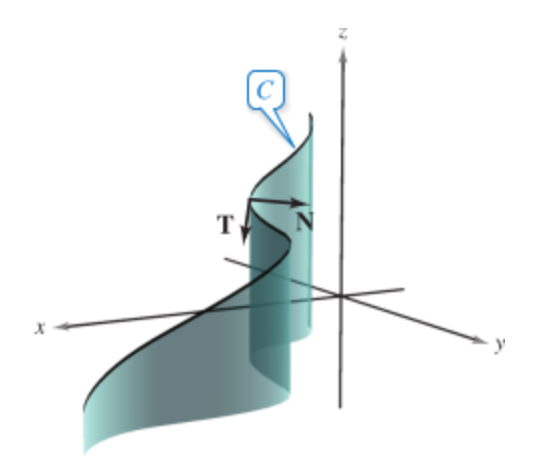
\includegraphics[width=0.4\textwidth]{tannorvec.png}&\parbox{0.5\textwidth}{\centering $\mathbf T\cdot\mathbf N = 0$\\(Not very intuitive though. Make sure you read the textbook and understand why it is true.)\vspace{10em}}
\end{tabular}
\end{frame}

\begin{frame}
\frametitle{Knowledge Checks}
What is the {\bf tangential} and the {\bf normal component} of the acceleration?\pause
\[
\mathbf a = a_T\mathbf T + a_N\mathbf N,\quad a_N > 0
\]
\pause
(Again, it's not very intuitive that $\mathbf a$ can be decomposed in this way in 3D space. Make sure you read the textbook and understand the proof.)
\pause

Key consequences:
\vskip -.5em

\begin{tabular}{cc}
\parbox{0.5\textwidth}{
\begin{align*}
a_T\mathbf T &= \operatorname{proj}_\mathbf v\mathbf a\\
a_N\mathbf N &= \mathbf a - \operatorname{proj}_\mathbf v \mathbf a\\
\mathbf N &= \frac{\mathbf a - \operatorname{proj}_\mathbf v \mathbf a}{a_N}\\ &= \frac{\mathbf a - \operatorname{proj}_\mathbf v \mathbf a}{\sqrt{\norm{\mathbf a}^2 - a_T^2}}\\& = \frac{\mathbf a - \operatorname{proj}_\mathbf v \mathbf a}{\norm{\mathbf a - \operatorname{proj}_\mathbf v \mathbf a}}  
\end{align*}
\vspace{12em}
}&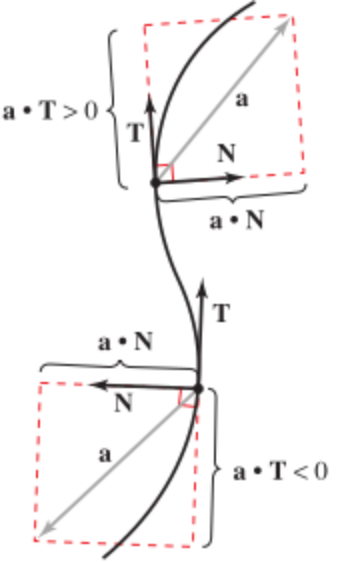
\includegraphics[width=.25\textwidth]{accelcomp.png}
\end{tabular}
\end{frame}

\end{document}